\chapter{Implementasi dan Pengujian}
\label{chap:implementasi_pengujian}

Bab ini menjelaskan mengenai lingkungan yang digunakan untuk melakukan implemantasi dan pengujian, masalah-masalah yang ditemui pada saat implementasi dan solusi yang dijalankan, pengujian yang dilakukan, baik pengujian fungsional maupun pengujian eksperimental, beserta hasilnya.

\section{Lingkungan Implementasi dan Pengujian}
\label{sec:lingkungan_implementasi_dan_pengujian}

Implementasi dan pengujian dilakukan pada laptop Asus N46VM dengan spesifikasi sebagai berikut:

\begin{itemize}
    \item{Sistem operasi: Windows 10}
    \item{Prosesor: Intel(R) Core(TM) i7-3610QM}
    \item{RAM: 12GB}
    \item{\textit{Network adapter}: Qualcomm Atheros AR9485WB-EG Wireless Network Adapter}
\end{itemize}

Implementasi dilakukan menggunakan bahasa pemrograman C\# dan IDE\footnote{Intergrated Develompent Environment} Microsoft Visual Studio Community 2015.

\section{Masalah Implementasi dan Solusinya}
\label{sec:masalah_implementasi}

Terdapat beberapa masalah implementasi yang membuat rancangan perangkat lunak tidak dapat sepenuhnya didasarkan pada hasil analisis, di antaranya:

\begin{itemize}
    \item{Fungsi window.external.notify tidak berperilaku sebagaimana yang diperkirakan. Fungsi ini diharapkan dapat dipanggil secara langsung di dalam kode javascript, namun ternyata tidak bisa. Setiap halaman yang ingin memanfaatkan fungsi ini harus didaftarkan pada Package.appxmanifest. Metode yang digunakan untuk mendapatkan hasil yang sama dengan fungsi yang diberikan oleh window.external.notify adalah dengan menggunakan kelas bertipe RuntimeComponent yang diizinkan untuk dapat diakses oleh JavaScript pada WebView. Kelas ini adalah ScriptNotifyHandler pada gambar \ref{fig:DetailedClassDiagram}.}
    \item{Fungsi window.open dan fungsi open tidak dapat dijalankan secara otomatis sehingga popup tidak muncul. Metode yang digunakan untuk mendapatkan hasil yang sama dari yang direncanakan sebelumnya adalah dengan melakukan \textit{override} fungsi window.open dan fungsi open pada saat halaman selesai dimuat, dan mengubungkannya dengan kelas ScriptNotifyHandler. Akan tetapi, metode ini masih kurang memadai karena kode JavaScript yang memanggil fungsi-fungsi tersebut pada saat halaman dimuat akan dieksekusi sebelum \textit{override} terjadi.}
\end{itemize}

Perancangan yang tertulis pada bab 4 sudah merupakan hasil revisi dari analisis masalah implementasi ini.



\section{Implementasi Antarmuka}
\label{sec:implementasi_antarmuka}

Implementasi antarmuka dibuat sesuai perancangan pada Bab 4. Antarmuka memiliki komponen utama yang berada di tengah yang dapat menampilkan pesan berhasil atau pesan-pesan lainnya, serta komponen di bagian bawah yang menampilkan \textit{settings} yang berisi daftar SSID WiFi yang sudah terekam pada perangkat lunak, serta tombol \textit{delete} untuk menghapus SSID yang dipilih dari daftar tersebut.

\begin{figure}[!htb]
    \centering
    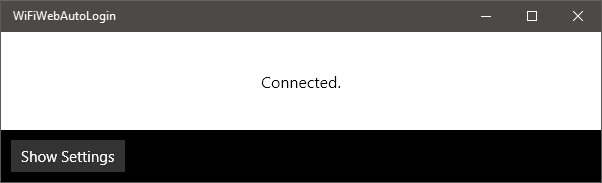
\includegraphics[scale=0.9]{Gambar/ui_hidden.png}
    \caption[Antarmuka dengan \textit{settings} yang tersembunyi.]{Antarmuka dengan \textit{settings} yang tersembunyi.} 
    \label{fig:ui_hidden}
\end{figure}

\begin{figure}[!htb]
    \centering
    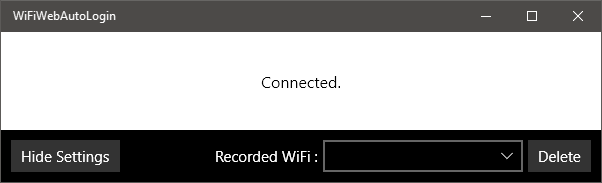
\includegraphics[scale=0.9]{Gambar/ui_shown.png}
    \caption[Antarmuka dengan \textit{settings} yang tampak.]{Antarmuka dengan \textit{settings} yang tampak.} 
    \label{fig:ui_shown}
\end{figure}

Gambar \ref{fig:ui_hidden} menampilkan antarmuka dengan \textit{settings} yang belum muncul dan gambar \ref{fig:ui_shown} menampilkan antamuka dengan \textit{settings} yang sudah muncul. \textit{Settings} akan tersembunyi pada saat antarmuka pertama kali muncul, dan akan muncul pada saat pengguna menekan tombol \textit{Show Settings}.



\section{Pengujian Fungsional}
\label{sec:pengujian_fungsional}

Pengujian fungsional dilakukan pada jaringan WiFi di kost di jalan Ciumbuleuit nomor 149, Bandung, dengan SSID "C149Net". Pengujian fungsional dilakukan pada tanggal 4 April 2017.

\subsection{Rencana Pengujian Fungsional}
\label{subsec:rencana_pengujian_fungsional}

Pengujian fungsional dilakukan menggunakan teknik \textit{black box}. Pengujian fungsional dilakukan untuk memastikan fungsi-fungsi utama dalam perangkat lunak sudah berjalan dengan baik. Fungsi-fungsi yang akan diuji mencakupi:

\begin{itemize}
    \item{Deteksi perubahan jaringan.}
    \item{Deteksi \textit{captive portal}.}
    \item{Login otomatis.}
\end{itemize}

Setiap fungsi yang diuji diberikan kasus pengujian positif dan pengujian negatif.

\subsection{Hasil Pengujian Fungsional}
\label{subsec:hasil_pengujian_fungsional}

Hasil-hasil pengujian fungsional adalah sebagai berikut:

\begin{itemize}
    \item{
        \textbf{Pengujian deteksi perubahan jaringan}
        
        \begin{itemize}
            \item{
                \textbf{Pengujian positif}\\
                \textbf{Kasus}: Menghubungkan komputer dengan WiFi yang terhubung dengan \textit{captive portal}.\\
                \textbf{Hasil yang diharapkan}: Muncul notifikasi.\\
                \textbf{Hasil yang didapatkan}: Muncul notifikasi "Network Detected" dengan pesan "Would you like to run WiFiWebAutoLogin?".\\
                \textbf{Kesimpulan}: Fungsi berjalan sesuai harapan.
            }
            \item{
                \textbf{Pengujian negatif}\\
                \textbf{Kasus}: Menghubungkan komputer dengan WiFi yang tidak terhubung dengan \textit{captive portal}.\\
                \textbf{Hasil yang diharapkan}: Tidak muncul notifikasi apapun.\\
                \textbf{Hasil yang didapatkan}: Tidak muncul notifikasi apapun.\\
                \textbf{Kesimpulan}: Fungsi berjalan sesuai harapan.
            }
        \end{itemize}
    }
    \item{
        \textbf{Pengujian deteksi \textit{captive portal}}
        
        \begin{itemize}
            \item{
                \textbf{Pengujian positif}\\
                \textbf{Kasus}: Menghubungkan komputer dengan WiFi yang terhubung dengan \textit{captive portal} dan menekan tombol "Yes" pada notifikasi.\\
                \textbf{Hasil yang diharapkan}: Muncul halaman login.\\
                \textbf{Hasil yang didapatkan}: Muncul halaman login \textit{captive portal}.\\
                \textbf{Kesimpulan}: Fungsi berjalan sesuai harapan.
            }
            \item{
                \textbf{Pengujian negatif}\\
                \textbf{Kasus}: Menghubungkan komputer dengan WiFi yang tidak terhubung dengan \textit{captive portal} maupun internet dan menekan tombol "Yes" pada notifikasi\\
                \textbf{Hasil yang diharapkan}: Muncul pesan \textit{timeout}.\\
                \textbf{Hasil yang didapatkan}: Muncul pesan "Operation timeout. Check your network connection.".\\
                \textbf{Kesimpulan}: Fungsi berjalan sesuai harapan.
            }
        \end{itemize}
    }
    \item{
        \textbf{Pengujian login otomatis}
        
        \begin{itemize}
            \item{
                \textbf{Pengujian positif}\\
                \textbf{Kasus}: Menghubungkan komputer dengan WiFi yang terhubung dengan \textit{captive portal} yang sudah pernah dijalankan login secara manual.\\
                \textbf{Hasil yang diharapkan}: Muncul pesan "Connected.".\\
                \textbf{Hasil yang didapatkan}: Muncul pesan "Executing recorded actions...", lalu setelah beberapa saat, muncul pesan "Connected.".\\
                \textbf{Kesimpulan}: Fungsi berjalan sesuai harapan.
            }
            \item{
                \textbf{Pengujian negatif}\\
                \textbf{Kasus}: Menghubungkan komputer dengan WiFi yang terhubung dengan \textit{captive portal} yang belum pernah dijalankan login secara manual.\\
                \textbf{Hasil yang diharapkan}: Muncul halaman login.\\
                \textbf{Hasil yang didapatkan}: Muncul halaman login \textit{captive portal}.\\
                \textbf{Kesimpulan}: Fungsi berjalan sesuai harapan.
            }
        \end{itemize}
    }
\end{itemize}



\section{Pengujian Eksperimental}
\label{sec:pengujian_eksperimental}

Pengujian eksperimental dilakukan untuk memeriksa apakah perangkat lunak dapat berjalan pada beragam \textit{captive portal}. Pengujian eksperimental dilakukan pada tanggal 5 April 2017.

\subsection{Rencana Pengujian Eksperimental}
\label{subsec:rencana_pengujian_eksperimental}

Pengujian eksperimental dilakukan pada \textit{captive portal} pada jaringan WiFi dengan SSID:

\begin{itemize}
    \item{\textit{C149Net} pada kost di jalan Ciumbuleuit nomor 149, Bandung.}
    \item{\textit{Starbucks@wifi.id} pada Starbucks Dipatiukur, Bandung.}
    \item{\textit{wifi.id} pada Starbucks Dipatiukur, Bandung.}
    \item{\textit{UNPAR9} pada gedung 10 Universitas Katolik Parahyangan, Bandung.}
    \item{\textit{FTIS.cisco} pada gedung 9 Universitas Katolik Parahyangan, Bandung.}
\end{itemize}

\subsection{Hasil Pengujian Eksperimental}
\label{subsec:hasil_pengujian_eksperimental}

Hasil pengujian eksperimental akan dijelaskan untuk setiap SSID yang diuji. Penjelasan berupa narasi hasil yang didapatkan berdasarkan langkah-langkah yang sama dengan pengujian fungsional \textit{black box}.

\subsubsection{Hasil Pengujian WiFi C149Net}
\label{subsubsec:C149Net}

Pengujian pada WiFi dengan SSID C149Net yang berlokasi pada kost di jalan Ciumbuleuit nomor 149, Bandung, mendapatkan hasil sesuai harapan. Notifikasi muncul pada saat WiFi pertama kali terhubung. Halaman login muncul setelah tombol "Yes" pada notifikasi ditekan. Setelah memasukkan \textit{username} dan \textit{password}, pesan "Connected." muncul. Jika informasi login sudah tersimpan, pesan "Connected." akan langsung muncul setelah menekan tombol "Yes" pada notifikasi.

\subsubsection{Hasil Pengujian WiFi Starbucks@wifi.id}
\label{subsubsec:starbucks_wifi_id}

Pengujian pada WiFi dengan SSID Starbucks@wifi.id yang berlokasi pada Starbucks Dipatiukur, Bandung, mendapatkan hasil sesuai harapan. Notifikasi muncul pada saat WiFi pertama kali terhubung. Halaman \textit{captive portal} muncul setelah tombol "Yes" pada notifikasi ditekan. Setelah menekan tombol "continue" pada halaman tersebut, lalu menekan tombol "lanjutkan" pada halaman selanjutnya, pesan "Connected." muncul. Jika informasi login sudah tersimpan, pesan "Connected." akan langsung muncul setelah menekan tombol "Yes" pada notifikasi.

\subsubsection{Hasil Pengujian WiFi wifi.id}
\label{subsubsec:wifi_id}

Pengujian pada WiFi dengan SSID wifi.id yang berlokasi pada Starbucks Dipatiukur, Bandung, mendapatkan hasil yang tidak sesuai harapan. Notifikasi muncul pada saat WiFi pertama kali terhubung. Halaman login muncul setelah tombol "Yes" pada notifikasi ditekan. Akan tetapi, login tidak dapat dilakukan karena perlu membeli voucher setiap kali ingin melakukan login.

\subsubsection{Hasil Pengujian WiFi UNPAR9}
\label{subsubsec:unpar9}

Pengujian pada WiFi dengan SSID UNPAR9 yang berlokasi pada gedung 10 Universitas Katolik Parahyangan, Bandung, mendapatkan hasil yang tidak sesuai harapan. Notifikasi muncul pada saat WiFi pertama kali terhubung. Halaman login muncul setelah tombol "Yes" pada notifikasi ditekan. Setelah login dilakukan, proses terhenti pada halaman \texttt{https://portal.unpar.ac.id/home}. Hal ini dikarenakan WiFi di Universitas Katolik Parahyangan menggunakan CAS\footnote{\textit{Central Authorization Service}}. Selain itu, CAS ini menggunakan \textit{pop-up} untuk menampilkan halaman \texttt{https://wireless.unpar.ac.id/status} dan halaman tersebut adalah halaman yang membuka popup yang menuju ke halaman tujuan. WebView pada UWP tidak memperbolehkan pemanggilan fungsi open(), window.open(), el.click() dan form.submit() yang bukan merupakan aksi langsung oleh pengguna. \textit{Override} tiap fungsi tersebut dimungkinkan setelah halaman selesai dimuat, namun itu berarti fungsi hasil \textit{override} tidak akan digunakan jika fungsi tersebut dipanggil pada saat halaman pertama kali dimuat. Hal ini mencakup \textit{onload event} dan script yang dipanggil langsung pada \textit{script tag} baik pada \textit{body} maupun \textit{head}.

\subsubsection{Hasil Pengujian WiFi FTIS.cisco}
\label{subsubsec:ftis_cisco}

Pengujian pada WiFi dengan SSID FTIS.cisco yang berlokasi pada gedung 9 Universitas Katolik Parahyangan, Bandung, mendapatkan hasil yang tidak sesuai harapan. Hal ini terjadi karena WiFi ini merupakan jaringan internal Fakultas Teknologi dan Sains yang menggunakan jaringan WiFi Universitas Katolik Parahyangan untuk akses internet. Proses terhenti pada halaman yang sama dengan WiFi UNPAR9 dan penyebab terjadinya hal ini juga sama dengan yang terjadi pada WiFi UNPAR9.